
%% bare_conf.tex
%% V1.4b
%% 2015/08/26
%% by Michael Shell
%% See:
%% http://www.michaelshell.org/
%% for current contact information.
%%
%% This is a skeleton file demonstrating the use of IEEEtran.cls
%% (requires IEEEtran.cls version 1.8b or later) with an IEEE
%% conference paper.
%%
%% Support sites:
%% http://www.michaelshell.org/tex/ieeetran/
%% http://www.ctan.org/pkg/ieeetran
%% and
%% http://www.ieee.org/

%%*************************************************************************
%% Legal Notice:
%% This code is offered as-is without any warranty either expressed or
%% implied; without even the implied warranty of MERCHANTABILITY or
%% FITNESS FOR A PARTICULAR PURPOSE! 
%% User assumes all risk.
%% In no event shall the IEEE or any contributor to this code be liable for
%% any damages or losses, including, but not limited to, incidental,
%% consequential, or any other damages, resulting from the use or misuse
%% of any information contained here.
%%
%% All comments are the opinions of their respective authors and are not
%% necessarily endorsed by the IEEE.
%%
%% This work is distributed under the LaTeX Project Public License (LPPL)
%% ( http://www.latex-project.org/ ) version 1.3, and may be freely used,
%% distributed and modified. A copy of the LPPL, version 1.3, is included
%% in the base LaTeX documentation of all distributions of LaTeX released
%% 2003/12/01 or later.
%% Retain all contribution notices and credits.
%% ** Modified files should be clearly indicated as such, including  **
%% ** renaming them and changing author support contact information. **
%%*************************************************************************


% *** Authors should verify (and, if needed, correct) their LaTeX system  ***
% *** with the testflow diagnostic prior to trusting their LaTeX platform ***
% *** with production work. The IEEE's font choices and paper sizes can   ***
% *** trigger bugs that do not appear when using other class files.       ***                          ***
% The testflow support page is at:
% http://www.michaelshell.org/tex/testflow/



\documentclass[conference]{IEEEtran}
% Some Computer Society conferences also require the compsoc mode option,
% but others use the standard conference format.
%
% If IEEEtran.cls has not been installed into the LaTeX system files,
% manually specify the path to it like:
% \documentclass[conference]{../sty/IEEEtran}





% Some very useful LaTeX packages include:
% (uncomment the ones you want to load)


% *** MISC UTILITY PACKAGES ***
%
%\usepackage{ifpdf}
% Heiko Oberdiek's ifpdf.sty is very useful if you need conditional
% compilation based on whether the output is pdf or dvi.
% usage:
% \ifpdf
%   % pdf code
% \else
%   % dvi code
% \fi
% The latest version of ifpdf.sty can be obtained from:
% http://www.ctan.org/pkg/ifpdf
% Also, note that IEEEtran.cls V1.7 and later provides a builtin
% \ifCLASSINFOpdf conditional that works the same way.
% When switching from latex to pdflatex and vice-versa, the compiler may
% have to be run twice to clear warning/error messages.






% *** CITATION PACKAGES ***
%
%\usepackage{cite}
% cite.sty was written by Donald Arseneau
% V1.6 and later of IEEEtran pre-defines the format of the cite.sty package
% \cite{} output to follow that of the IEEE. Loading the cite package will
% result in citation numbers being automatically sorted and properly
% "compressed/ranged". e.g., [1], [9], [2], [7], [5], [6] without using
% cite.sty will become [1], [2], [5]--[7], [9] using cite.sty. cite.sty's
% \cite will automatically add leading space, if needed. Use cite.sty's
% noadjust option (cite.sty V3.8 and later) if you want to turn this off
% such as if a citation ever needs to be enclosed in parenthesis.
% cite.sty is already installed on most LaTeX systems. Be sure and use
% version 5.0 (2009-03-20) and later if using hyperref.sty.
% The latest version can be obtained at:
% http://www.ctan.org/pkg/cite
% The documentation is contained in the cite.sty file itself.






% *** GRAPHICS RELATED PACKAGES ***
%
\ifCLASSINFOpdf
  % \usepackage[pdftex]{graphicx}
  % declare the path(s) where your graphic files are
  % \graphicspath{{../pdf/}{../jpeg/}}
  % and their extensions so you won't have to specify these with
  % every instance of \includegraphics
  % \DeclareGraphicsExtensions{.pdf,.jpeg,.png}
\else
  % or other class option (dvipsone, dvipdf, if not using dvips). graphicx
  % will default to the driver specified in the system graphics.cfg if no
  % driver is specified.
  % \usepackage[dvips]{graphicx}
  % declare the path(s) where your graphic files are
  % \graphicspath{{../eps/}}
  % and their extensions so you won't have to specify these with
  % every instance of \includegraphics
  % \DeclareGraphicsExtensions{.eps}
\fi
% graphicx was written by David Carlisle and Sebastian Rahtz. It is
% required if you want graphics, photos, etc. graphicx.sty is already
% installed on most LaTeX systems. The latest version and documentation
% can be obtained at: 
% http://www.ctan.org/pkg/graphicx
% Another good source of documentation is "Using Imported Graphics in
% LaTeX2e" by Keith Reckdahl which can be found at:
% http://www.ctan.org/pkg/epslatex
%
% latex, and pdflatex in dvi mode, support graphics in encapsulated
% postscript (.eps) format. pdflatex in pdf mode supports graphics
% in .pdf, .jpeg, .png and .mps (metapost) formats. Users should ensure
% that all non-photo figures use a vector format (.eps, .pdf, .mps) and
% not a bitmapped formats (.jpeg, .png). The IEEE frowns on bitmapped formats
% which can result in "jaggedy"/blurry rendering of lines and letters as
% well as large increases in file sizes.
%
% You can find documentation about the pdfTeX application at:
% http://www.tug.org/applications/pdftex





% *** MATH PACKAGES ***
%
%\usepackage{amsmath}
% A popular package from the American Mathematical Society that provides
% many useful and powerful commands for dealing with mathematics.
%
% Note that the amsmath package sets \interdisplaylinepenalty to 10000
% thus preventing page breaks from occurring within multiline equations. Use:
%\interdisplaylinepenalty=2500
% after loading amsmath to restore such page breaks as IEEEtran.cls normally
% does. amsmath.sty is already installed on most LaTeX systems. The latest
% version and documentation can be obtained at:
% http://www.ctan.org/pkg/amsmath





% *** SPECIALIZED LIST PACKAGES ***
%
%\usepackage{algorithmic}
% algorithmic.sty was written by Peter Williams and Rogerio Brito.
% This package provides an algorithmic environment fo describing algorithms.
% You can use the algorithmic environment in-text or within a figure
% environment to provide for a floating algorithm. Do NOT use the algorithm
% floating environment provided by algorithm.sty (by the same authors) or
% algorithm2e.sty (by Christophe Fiorio) as the IEEE does not use dedicated
% algorithm float types and packages that provide these will not provide
% correct IEEE style captions. The latest version and documentation of
% algorithmic.sty can be obtained at:
% http://www.ctan.org/pkg/algorithms
% Also of interest may be the (relatively newer and more customizable)
% algorithmicx.sty package by Szasz Janos:
% http://www.ctan.org/pkg/algorithmicx




% *** ALIGNMENT PACKAGES ***
%
%\usepackage{array}
% Frank Mittelbach's and David Carlisle's array.sty patches and improves
% the standard LaTeX2e array and tabular environments to provide better
% appearance and additional user controls. As the default LaTeX2e table
% generation code is lacking to the point of almost being broken with
% respect to the quality of the end results, all users are strongly
% advised to use an enhanced (at the very least that provided by array.sty)
% set of table tools. array.sty is already installed on most systems. The
% latest version and documentation can be obtained at:
% http://www.ctan.org/pkg/array


% IEEEtran contains the IEEEeqnarray family of commands that can be used to
% generate multiline equations as well as matrices, tables, etc., of high
% quality.




% *** SUBFIGURE PACKAGES ***
%\ifCLASSOPTIONcompsoc
%  \usepackage[caption=false,font=normalsize,labelfont=sf,textfont=sf]{subfig}
%\else
%  \usepackage[caption=false,font=footnotesize]{subfig}
%\fi
% subfig.sty, written by Steven Douglas Cochran, is the modern replacement
% for subfigure.sty, the latter of which is no longer maintained and is
% incompatible with some LaTeX packages including fixltx2e. However,
% subfig.sty requires and automatically loads Axel Sommerfeldt's caption.sty
% which will override IEEEtran.cls' handling of captions and this will result
% in non-IEEE style figure/table captions. To prevent this problem, be sure
% and invoke subfig.sty's "caption=false" package option (available since
% subfig.sty version 1.3, 2005/06/28) as this is will preserve IEEEtran.cls
% handling of captions.
% Note that the Computer Society format requires a larger sans serif font
% than the serif footnote size font used in traditional IEEE formatting
% and thus the need to invoke different subfig.sty package options depending
% on whether compsoc mode has been enabled.
%
% The latest version and documentation of subfig.sty can be obtained at:
% http://www.ctan.org/pkg/subfig




% *** FLOAT PACKAGES ***
%
%\usepackage{fixltx2e}
% fixltx2e, the successor to the earlier fix2col.sty, was written by
% Frank Mittelbach and David Carlisle. This package corrects a few problems
% in the LaTeX2e kernel, the most notable of which is that in current
% LaTeX2e releases, the ordering of single and double column floats is not
% guaranteed to be preserved. Thus, an unpatched LaTeX2e can allow a
% single column figure to be placed prior to an earlier double column
% figure.
% Be aware that LaTeX2e kernels dated 2015 and later have fixltx2e.sty's
% corrections already built into the system in which case a warning will
% be issued if an attempt is made to load fixltx2e.sty as it is no longer
% needed.
% The latest version and documentation can be found at:
% http://www.ctan.org/pkg/fixltx2e


%\usepackage{stfloats}
% stfloats.sty was written by Sigitas Tolusis. This package gives LaTeX2e
% the ability to do double column floats at the bottom of the page as well
% as the top. (e.g., "\begin{figure*}[!b]" is not normally possible in
% LaTeX2e). It also provides a command:
%\fnbelowfloat
% to enable the placement of footnotes below bottom floats (the standard
% LaTeX2e kernel puts them above bottom floats). This is an invasive package
% which rewrites many portions of the LaTeX2e float routines. It may not work
% with other packages that modify the LaTeX2e float routines. The latest
% version and documentation can be obtained at:
% http://www.ctan.org/pkg/stfloats
% Do not use the stfloats baselinefloat ability as the IEEE does not allow
% \baselineskip to stretch. Authors submitting work to the IEEE should note
% that the IEEE rarely uses double column equations and that authors should try
% to avoid such use. Do not be tempted to use the cuted.sty or midfloat.sty
% packages (also by Sigitas Tolusis) as the IEEE does not format its papers in
% such ways.
% Do not attempt to use stfloats with fixltx2e as they are incompatible.
% Instead, use Morten Hogholm'a dblfloatfix which combines the features
% of both fixltx2e and stfloats:
%
% \usepackage{dblfloatfix}
% The latest version can be found at:
% http://www.ctan.org/pkg/dblfloatfix




% *** PDF, URL AND HYPERLINK PACKAGES ***
%
%\usepackage{url}
% url.sty was written by Donald Arseneau. It provides better support for
% handling and breaking URLs. url.sty is already installed on most LaTeX
% systems. The latest version and documentation can be obtained at:
% http://www.ctan.org/pkg/url
% Basically, \url{my_url_here}.




% *** Do not adjust lengths that control margins, column widths, etc. ***
% *** Do not use packages that alter fonts (such as pslatex).         ***
% There should be no need to do such things with IEEEtran.cls V1.6 and later.
% (Unless specifically asked to do so by the journal or conference you plan
% to submit to, of course. )

\usepackage{tabularx}
\usepackage{lipsum}
\usepackage{blindtext}
\usepackage{graphicx}
\usepackage{url}
\usepackage[usenames,dvipsnames,svgnames,table]{xcolor}


\newcommand{\ck}[1]{\textcolor{red}{#1}}

\newcolumntype{K}[1]{>{\centering\arraybackslash}p{#1}}



% correct bad hyphenation here
\hyphenation{op-tical net-works semi-conduc-tor}


\begin{document}

\title{Old is Still Gold: A Comparison of Cyber and Regular Consumer Fraud in The United States}


% author names and affiliations
\author{\IEEEauthorblockN{Mohammad Taha Khan and Chris Kanich}
\IEEEauthorblockA{Department of Computer Science, University of Illinois at Chicago\\taha@cs.uic.edu, ckanich@uic.edu}}

% make the title area
\maketitle

% As a general rule, do not put math, special symbols or citations
% in the abstract
\begin{abstract}

While cybercrime is a relatively recent human invention, fraudulent activity
has a much longer history. Understanding the extent to which cybercrime is fundamentally different from, or similar to, traditional fraudulent activity is the first step toward being able to effectively combat it. This paper investigates the differences in fraud
reporting and targeting among United States based consumers by comparing
fraudulent activity mediated by the Internet with traditional forms of
fraud. By partitioning the FTC Consumer Sentinel complaint dataset into
cyber and traditional categories, we summarize the difference in fraud
trends across time, distance and location metrics.We also evaluate fraud
variations across different ethnic and socio-economic factors. Our findings
suggest that both categories of frauds experience an overall decrease during
the holiday season. Individuals who are victimized via traditional methods
are more likely to complain using traditional methods, while a majority of
cyber victims submit fraud complaints online. By evaluating the top frauds
in each category, we demonstrate how traditional fraudsters have evolved in
their methodologies to execute scams on the Internet that were initially
perpetrated through traditional means.

\end{abstract}

\section{Introduction}

In the United States, a total of more than 25 million people are victims of frauds per year \cite{anderson2013consumer}. These deceptive scams are a major cause of economic damages to users, not to mention the added externalities of wasted time and stress. Such illicit practices have been a part of the underground economy for quite a while. Initially, individuals were tricked by scam calls, in-person fraudsters or snail mail, however, the rise of the Internet has provided fraudulent entities with a more streamlined exposure to the overall population. According to a Javelin study in 2017, identity frauds hit a record high, targeting 15.4 million victims in the United States \cite{identiytheftonline}. The findings indicated that individuals with an online presence were more susceptible to possibility of theft. Another recent study released by the  Federal Trade Commission (FTC) reported that debt collection, identity theft, and impostor scams contributed towards 56\% of the total frauds complaints in 2015 \cite{ftcpress2016} . With the number of Internet users on the rise, the number of cyber frauds is likely to increase over the next couple of years \cite{perharassment}. To deal with this rising situation, the Federal Bureau of Investigation (FBI), has also been actively involved in addressing this issue. Their complaint portal, known as the IC3 is specifically designed to record complaints on Internet-based fraudulent practices \cite{fbiic3}. This emerging trend of deceptive practices necessitates their study in order to evaluate and mitigate the harm caused to victims.

This paper evaluates the nature of consumer fraud in the United States. Our work provides a comparison between cyber and traditional frauds. We categorize cyber frauds as all those deceptive practices that victimize users online, while regular (or traditional) ones comprise of frauds that target individuals over the phone, with mail, or in-person. While we understand that online scams \cite{miramirkhani2016dial} are a major focus of today's research, our comparison based approach allows us to better understand how they differ from traditional fraud methods. It also enables us to independently evaluate trends in traditional frauds and to see whether fraudsters are adopting online mechanisms to target more individuals. This combined analysis enables us to provide strategic suggestions in means to develop better fraud reduction methodologies.

To evaluate fraud trends, we use the FTC's Consumer Sentinel database, a dataset of complaints from the year 2013 and 2014. We also collect demographic information from the US Census Bureau \cite{uscensus}. In addition to data collection, we devise a calibration methodology to identify and separate cyber frauds from regular ones in the complaint dataset. 

Our work provides three main contributions. First, we evaluate the distinctive trends prevalent in cyber and regular frauds in the dataset. This encompasses their reporting numbers and methods, the nature of frauds which are more common in each specific category as well as the insights on the fraudsters who carry out these specific deceptive activities. Secondly, we look at ethnic, age, education, and employment demographics in each specific category and evaluate if certain individuals are more likely to report. Finally, based on our findings we suggest measures that can be taken into account by regulatory agencies to reduce overall fraud in the United States.

The rest of the paper is structured as follows, section \ref{related} provides a comprehensive overview of the relevant work. In section \ref{data-cal}, we elaborate on features of the datasets used in our analysis along with a description of our calibration methodology. Section \ref{eval} summarizes our findings from the data, followed by our suggestions to regulatory agencies in \ref{discussion}. We conclude our work in section \ref{conclusion} and discuss avenues of future research.


\section{Related Work}\label{related}


\begin{table*}[h]
\noindent
\centering
\begin{tabular}{K{0.2\linewidth}|p{0.7\linewidth}}
\hline
\multicolumn{1}{c}{\bfseries Data Field} & \multicolumn{1}{c}{\bfseries Field Description}
\\ 
\hline
\hline
Agency Name & The complaint collection agencies associated with the FTC.\\
\hline
Zip code Information & The zip code of the victim and the fraudulent entity.\\
%This provided us with low level granularity for analysis, however, the latter was only available for a subset of the complaints\\
\hline
Contact Method & The primary channel used by the fraudulent entity to contact the victim e.g. Internet, phone, mail.\\
\hline
Fraud Description & Nature of the fraud, and its type e.g. credit card, fake product, debt collection.\\
\hline
Occurrence \&
 Reporting Date & The dates when the fraud initially occurred and the date on which is was reported.
\\
\hline
\end{tabular}
\vspace{8pt}
\caption{data field primarily used for data calibration and analysis}\label{ftcdata}
\vspace{-20pt}
\end{table*}

As our work evaluates both cyber as well as regular frauds, we provide related work that encompasses both categories. Before the Internet became a primary hub of economic and social activity, researchers measured \cite{clarke2001controlling} and developed techniques based on statistical models \cite{brause1999neural, moreau1997detection, bolton2002statistical} to detect phone and credit card based frauds. In the past few years,  research evaluations have shifted focus towards cyber activity \cite{ablon2016consumer, piper2002, ionescu2011fraud, howard2007cyber, snyder2015no} due to the increased Internet usage trends for sensitive activities and its increased potential for harm.

Even though term \emph{"cyber fraud"} is usually associated with Computer Science, its recent socio-economic impact has motivated researchers in Economics, Law, and Finance to explore solutions by incorporating methodologies specific to their areas. Ionescu et al. characterize the types and sources of cyber financial frauds in global digital networks \cite{ionescu2011fraud}. The authors suggest the involvement of all stakeholders and employees through awareness and training to contain and reduce fraud. Similarly, Howard et al. study malicious code attacks against financial networks and suggest technical detection and mitigation techniques for financial infrastructure \cite{howard2007cyber} . Studies also show how the cyber criminals have several potential advantages over their opposing law enforcement agencies and suggest some practical steps to even out the differential gap \cite{piper2002}.

Due to an increase in the overall concern for online fraudulent activity, there has also been state-sponsored research that measures the impact of fraud. Smyth et al. measure the extent of cyber fraud in Canada in 2011 \cite{smyth2011measuring}. Their work indicates that a major chunk of frauds does not get recorded and hence the suggest a need for a sentinel to record fraud data, similar to the FTC complaint center in the US.

Another significant area of research focuses on understanding the demographics of fraud victims \cite{JOCA:JOCA1}. A recent FTC Report \cite{raval2016determines} quantifies complaint rates across different ethnic and education groups in the US. Garrett et al also look at how demographics affect the likelihood of an individual to complain about fraud \cite{garrett2010consumers}. Researchers have also focused on studying the reactions of the victims of an online data breach \cite{ablon2016consumer}. They categorize their results in different income, education, age, and ethnic groups. Such research aims to provide organizations with informed insight to better develop policies for consumer rights protection.

Contrary to previous research, which individually studies cyber or regular fraud, our work provides a unique angle of evaluation, by comparison of both fraud types. We evaluate characteristics for both types of cyber and regular frauds and their demographic trends.
\section{Data and Calibration} \label{data-cal}

In this section, we explain the characteristics of our datasets and the sources they were obtained from. We also provide insight into the essential processing and calibration methodology that we incorporate to classify and filter the data for a fair evaluation of our questions.


\subsection{Data Description}

\subsubsection{FTC Complaint Dataset}

\begin{table}[h]
\centering
\begin{tabular}{c|c}
\hline
{\bfseries Description} & \multicolumn{1}{c}{\bfseries Value}
\\
\hline
\hline
\% Cyber Complaints &52.1\\
\hline
\% Regular Complaints & 47.9\\
\hline
Month with Most Complaints & July 2013\\
\hline
Month with Least Complaints & Feb 2013\\
\hline
\end{tabular}
\vspace{8pt}
\caption{Summary Statistics of the FTC dataset}\label{summary_stats}
\vspace{-10pt}
\end{table}


The primary dataset we use for our evaluation is a corpus of the complaint logs collected between the months of Jan 2013 to June 2014 at agencies within the US and reported to the FTC\footnote{This data was obtained from the directly from the FTC under the Freedom of Information Act (FOIA).}. The Dataset is comprised of 865K complaints aggregated for cyber as well as regular fraud. Agencies responsible for collecting these logs provide online portals, phone or in-person reporting services. Inconsistent reporting semantics is an associated challenge with multiple data collection sources. While the FTC data is calibrated to a fair extent, to ensure the accuracy of our results, we perform an initial data consistency parse to exclude irrelevant outliers from the aggregated dataset. Table \ref{ftcdata} shows the fields of the used dataset along with their description. While the original dataset has several fields, for reader convenience and brevity, we only include the relevant ones form the basis our analysis. we also provide summary statistics of the data in table \ref{summary_stats}.
\\

\subsubsection{US Census Datasets}
Zip code information in our complaint dataset allows us to perform demographic analysis of the frauds. We obtain the demographic information associated with zip codes available at the US Census Bureau website \cite{uscensus}. The specific information that we collect is stated below:

\begin{itemize}
\vspace{8pt}
  \item Population density per zip code
  \item Education and income data \footnote{We obtained education data from an aggregator of US demographics \cite{zipatlas}.}
  \item Age statistics
  \item Race and ethnic information
  \vspace{8pt}
\end{itemize}

As zip codes provide a low-level granularity, to aggregate adjacent zip codes we obtain the Zip codes to the metropolitan Statistical Area (MSA) mappings from \cite{uslaborstats}. MSA are essentially groups of geographically connected zip codes that demonstrate strong social and economic linkage. While there are more than 40,000 zip codes in the United States there are only 382 distinct MSAs \cite{uscensus}. While our analysis in section \ref{demographic_analysis} aggregates different demographics based on zip codes, we incorporate the use of MSAs while performing location based evaluations in section \ref{fraudser_locations}. This essentially allows us to cluster the zip codes and associate a named location with them. This aggregation also helps mitigate any bias caused by an anomalous outlier zip code.

\subsection{Calibration Methodology}

One of the major fundamentals of our comparison is accurate tagging of each complaint as either cyber or regular fraud. While having a limited view of the fraud description, this paper takes a \emph{best effort} calibration approach to differentiate between the two types of frauds. To perform this calibration we use the \textbf{Contact Method} and \textbf{Fraud Description} fields from Table \ref{ftcdata}. Initially, we manually classify all contact methods and descriptions as either cyber or regular. We then flag a complaint as cyber if the victim's primary contact method was through online media; these are primarily websites, social networks, email, and IM. For the remainder of the complaints, we look at the description. If the complaint description involves something associated with the Internet, we classify it as a cyber fraud regardless of how the victim was initially approached. For instance, frauds, in which an individual is contacted via phone and requested to perform certain actions on their computer e.g. visiting a certain website, will be categorized as cyber. While this is a sophisticated technique that involves phone communication, the actual fraud hinges on the victim performing specific actions online, making it cyber nature. Figure \ref{classify} provides a visualization of our keyword classification methodology. This process provides us with two distinct categories and enables a fair comparison of the frauds.   

\begin{figure}[t]
\centering
  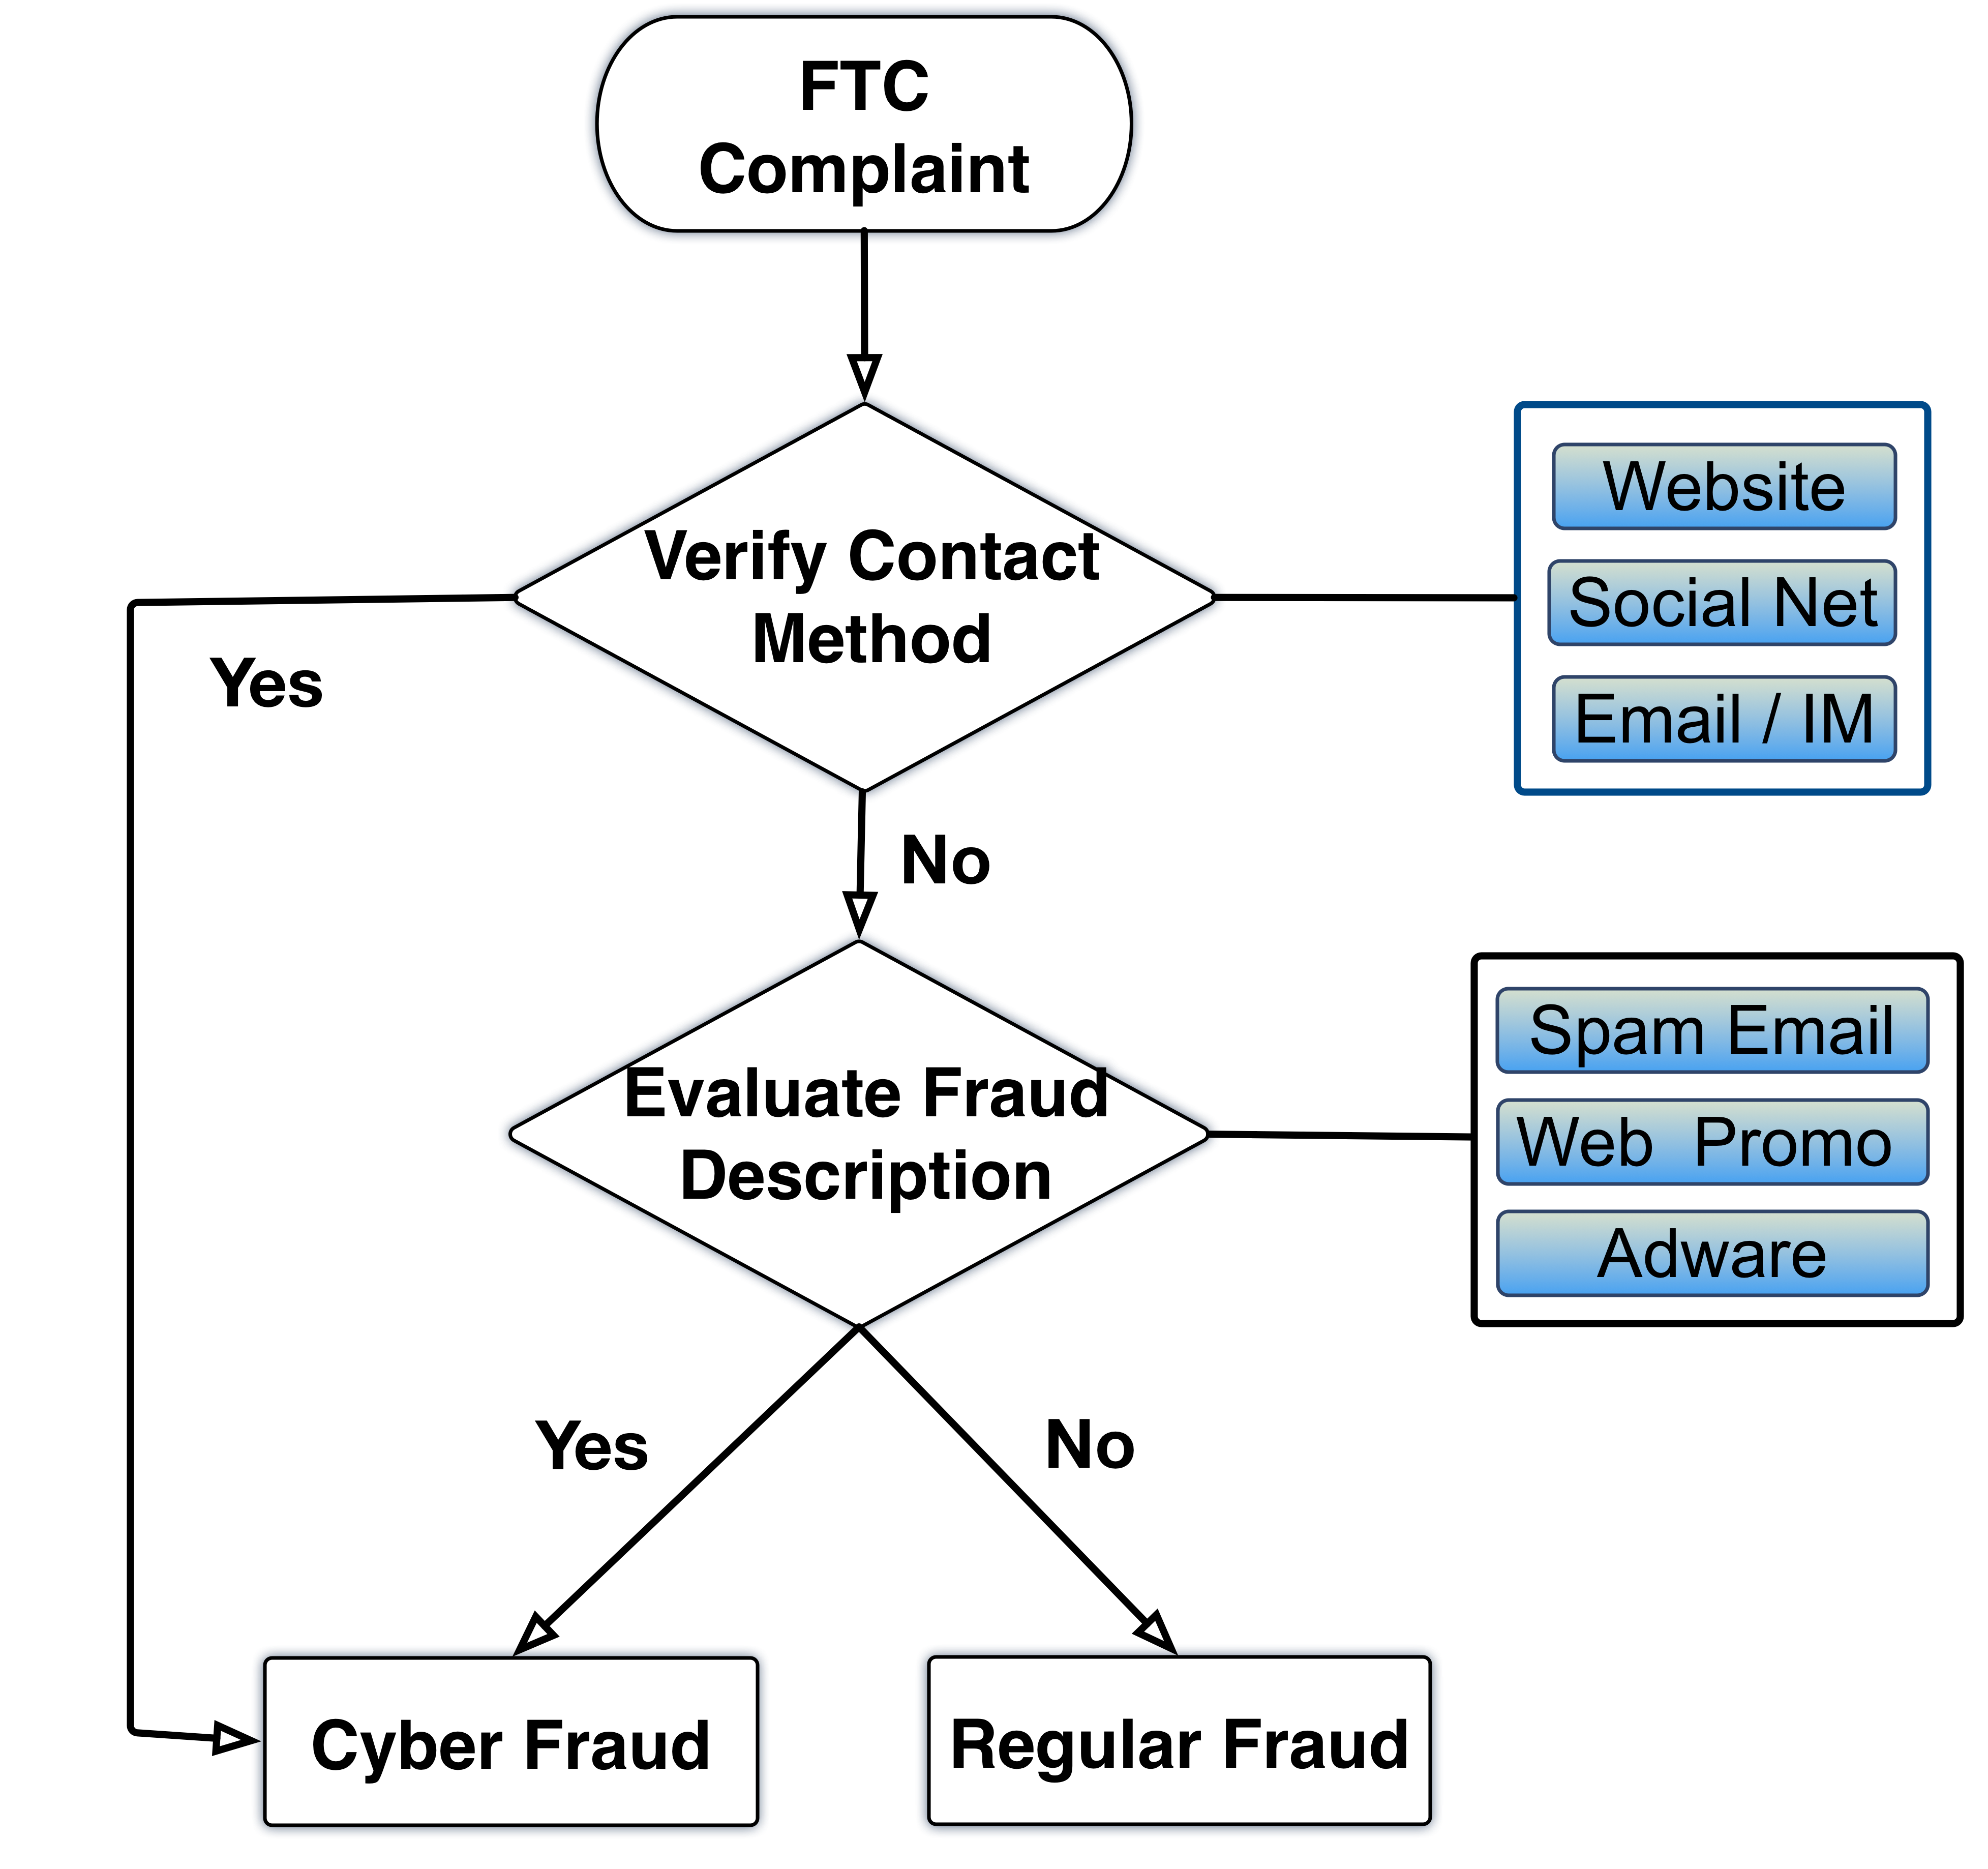
\includegraphics[scale=0.28]{graphics/methodology.png}
  \caption{Methodology for classifying cyber and regular frauds.}
  \label{classify}
\end{figure}

\section{Evaluation}\label{eval}

	
Having the categorized dataset, we aim to answer the primary question of how cyber and regular fraud compare to each other Based on the auxiliary information in the  FTC dataset, combined with the informative fields from secondary sources, we are able to explore various data dimensions for our cpmparison. First, we look at how cyber and regular crimes vary across the different times of the year. We then aim to understand the distribution of cyber and regular frauds across victims. We also compare the reaction of the targeted individuals by evaluating their respective reporting methods and reaction time. Similarly, we explore if fraudsters of cyber and regular frauds have certain distinguishable characteristics. Finally, we provide an in-depth comparison of various demographics for the two fraud types.


\subsection{Fraud Variation over Time}\label{var_time}



We initially perform a temporal analysis of the 15-month dataset to evaluate how the fraud reporting varies over time and explore when a certain type of frauds is more likely to be reported. We use the reporting date as an estimate of fraud count on that specific date. While the overall rate of fraud remains consistent, we observe a significant reduction in reporting in the winter holiday season. To investigate this, we select two distinct, 20 day periods in the dataset; we label them as \textbf{Working} (Aug, 15  to Sept, 5) and \textbf{Holiday} (Dec 15, to Jan, 5). Figure \ref{temporal} shows the variation of cyber and regular frauds within the two specific time periods. We observe a significant drop in the frauds during the holiday time period. Individually, cyber fraud decreases by 26\% while regular fraud decreases by a much larger value of 56\%. Our analysis is based on the conservative assumption that, reporting count on a date positively correlates with the number of frauds and there is not a significant reporting delay between the crime and reporting dates. We validate this in figure \ref{cdffig} (a), which shows that approximately 70\% of reporting dates are within a week of the date when the incident occurred, we also suggest some associated limitations to this approach in section \ref{reaction_time}. We also believe that the larger decrease in regular frauds is an overestimate as result of a bias that we explain using additional statistical findings from the next section.



\begin{figure}[t]
\centering
  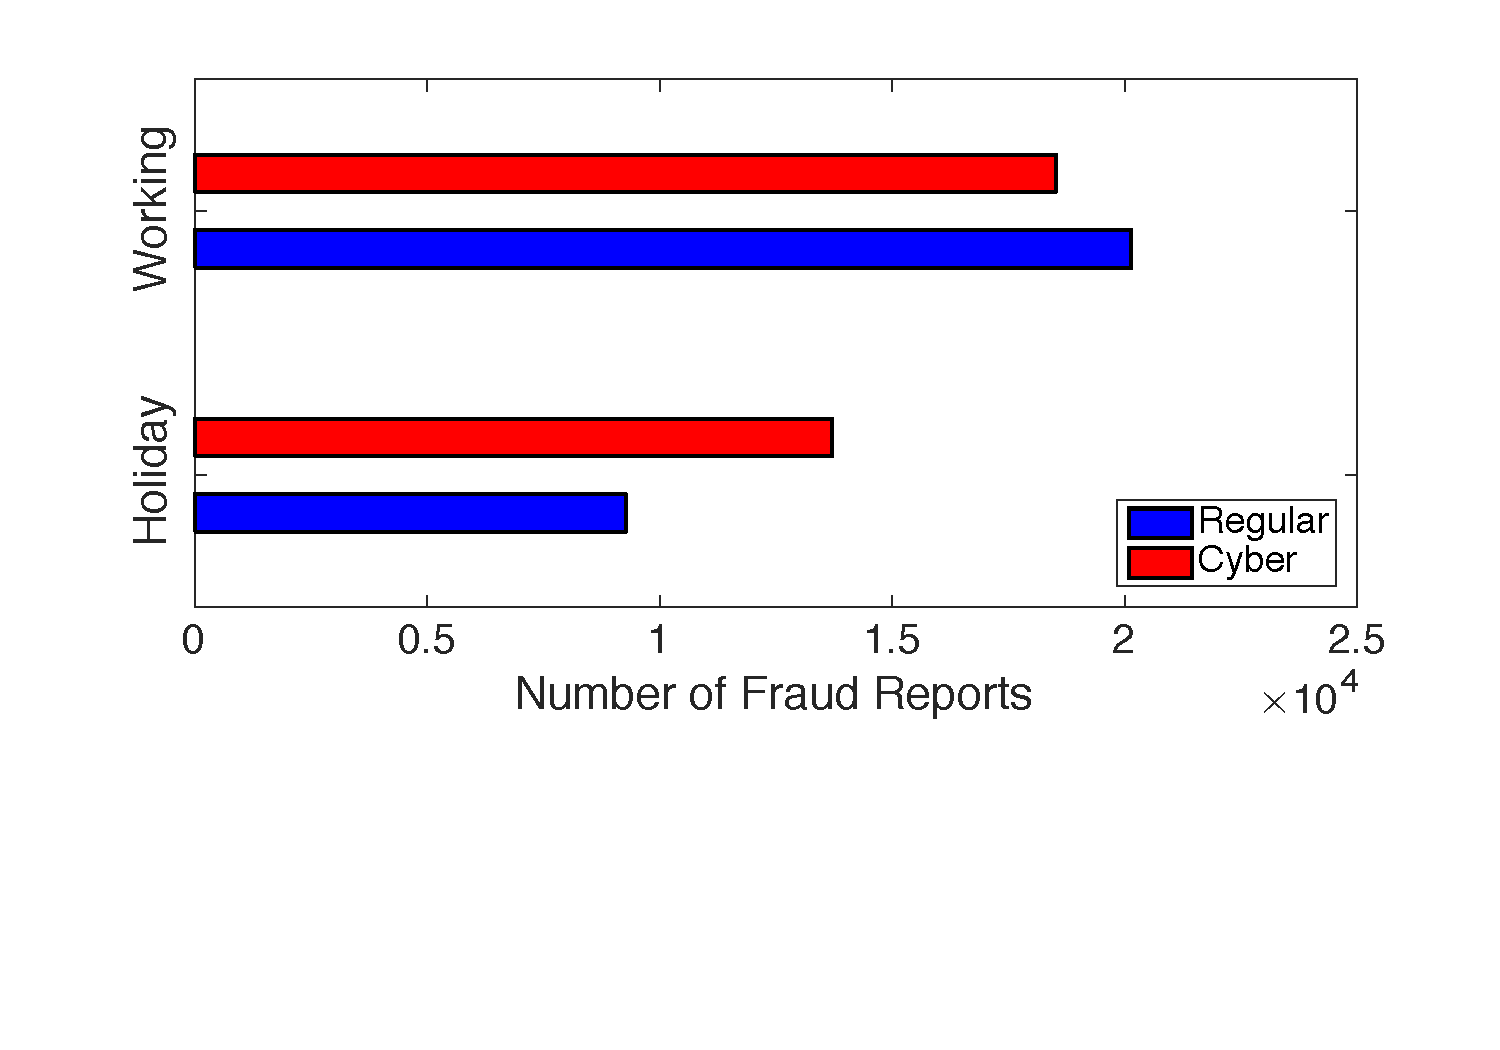
\includegraphics[scale=0.35]{graphics/reg_vs_holiday.pdf}
  \caption{Fraud reporting incidence during regular and holiday season}
  \label{temporal}
\end{figure}


\subsection{Fraud Reporting Methods}\label{reportingmethods}


Consumers have the ability to report complaints to the FTC via several methods and agencies. We aggregate the 26 complaint collecting entities into online and offline categories. For instance, reports made via the Internet complaint center or the FTC complaint assistant are tagged as online, while the ones issued to the FTC call center, publisher clearing house, attorneys general, or other regulatory institutions are categorized as offline. Figure \ref{reportingfig} provides the distribution of how individuals opt to report cyber and regular crimes. Approximately 82\% of cyber fraud victims used an online complaint facility, and 63\% of regular fraud victims reported via offline methods.

We observe that a major chunk of regular frauds is reported to offline institutions, which have reduced operation during holidays. We believe this significantly contributes to the reduction bias of the value of regular frauds in figure \ref{temporal}. 


 \begin{figure}[t]
\centering
  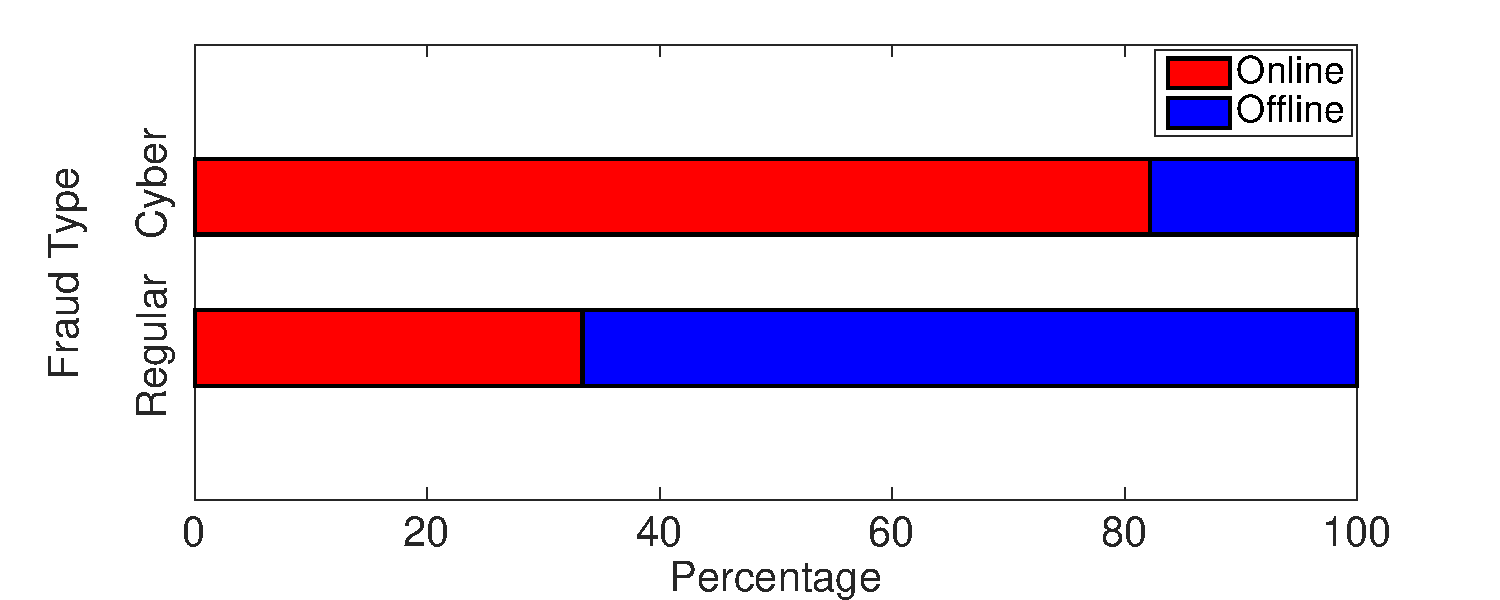
\includegraphics[scale=0.35]{graphics/reporting_methods.pdf}
  \caption{Distribution of reporting methods for frauds}
  \label{reportingfig}
\end{figure}



To further validate this, we perform a two-sample t-test over the distribution of fraud reports for both cyber and regular frauds. The compared distributions belong to the working and holiday period explained in section \ref{var_time}. Our null hypothesis assumes that both time periods belong to the same reporting pool. The statistically significant \emph{p-value} for regular frauds in table \ref{ttest} suggests in favor of the alternative hypothesis, hence validating our assumed bias for a decrease in regular frauds. Additionally, we also calculate the percent increase in reporting between the last 10 holidays and 10 working days right after. While cyber reports only increase by 37\% the increase in regular fraud reports is a staggering 104\%. The ratio of increases is in line with the proportions (17:66) for offline reporting methods used by cyber and regular fraud victims. We believe that while both types of frauds experience a decrease, the decrease in cyber frauds represents a more accurate trend. These derived insights enable us to suggest more meaningful measures in section \ref{discussion} to deal with consumer fraud.




\vspace{-8pt}

\begin{table}[h]
\centering
\begin{tabular}{cc}
\hline
\multicolumn{1}{c}{\bfseries Fraud Type} & \multicolumn{1}{c}{\bfseries \emph{p-value}}
\\
\hline
\hline
Cyber & 0.014\\
\hline
Regular & 0.003\\
\hline
\end{tabular}
\vspace{8pt}
\caption{t-test results for frauds across different time periods}\label{ttest}
\vspace{-10pt}
\end{table}



\subsection{Consumer Reaction Time}\label{reaction_time}

Here we evaluate on how quickly do victims of a fraud react and report the incident. Figure \ref{cdffig} (a) shows the CDF of the number of days between the date when the fraud occurred and when in was first reported to the FTC. We do not observe any difference between the reaction time trends of cyber and regular fraud victims. The graph shows that for both fraud categories, almost 30\% of the individuals take more than a week to respond. We believe that this provides ample time window for fraudsters to maliciously act on the assets acquired from individuals. This increased delay can also be a result of individuals discovering they were victimized by a fraud at a later date than the actual incident. One example would be a credit card theft when the victims only recognize the breach after they see an unauthorized transaction. Unfortunately, we do have enough information in the dataset to normalize in against such a situation in practice.

\begin{table}[h]
\centering
\begin{tabular}{c|c||c|c}
\hline
\bfseries Cyber & \bfseries \% & \bfseries Regular & \bfseries \% \\
\hline
\hline
Online Shopping \& Sales & 14.1 & Impostor Fraud & 29.8\\
\hline
Impostor Fraud & 10.8 & Telemarketing & 20.1\\
\hline
Unsolicited Email & 7.71 & Debt Collection & 16.1\\
\hline
Counterfeit Check Scams	 & 7.40 & Prizes \& Sweepstakes & 15.5 \\
\hline
Prizes \& Sweepstakes & 7.40 & Grants \& Credit Loans & 4.14\\
\hline
\hline
\end{tabular}
\vspace{8pt}
\caption{Top Fraud Descriptions}\label{topfrauds}
\vspace{-15pt}
\end{table}




\begin{figure}[t]
\centering
  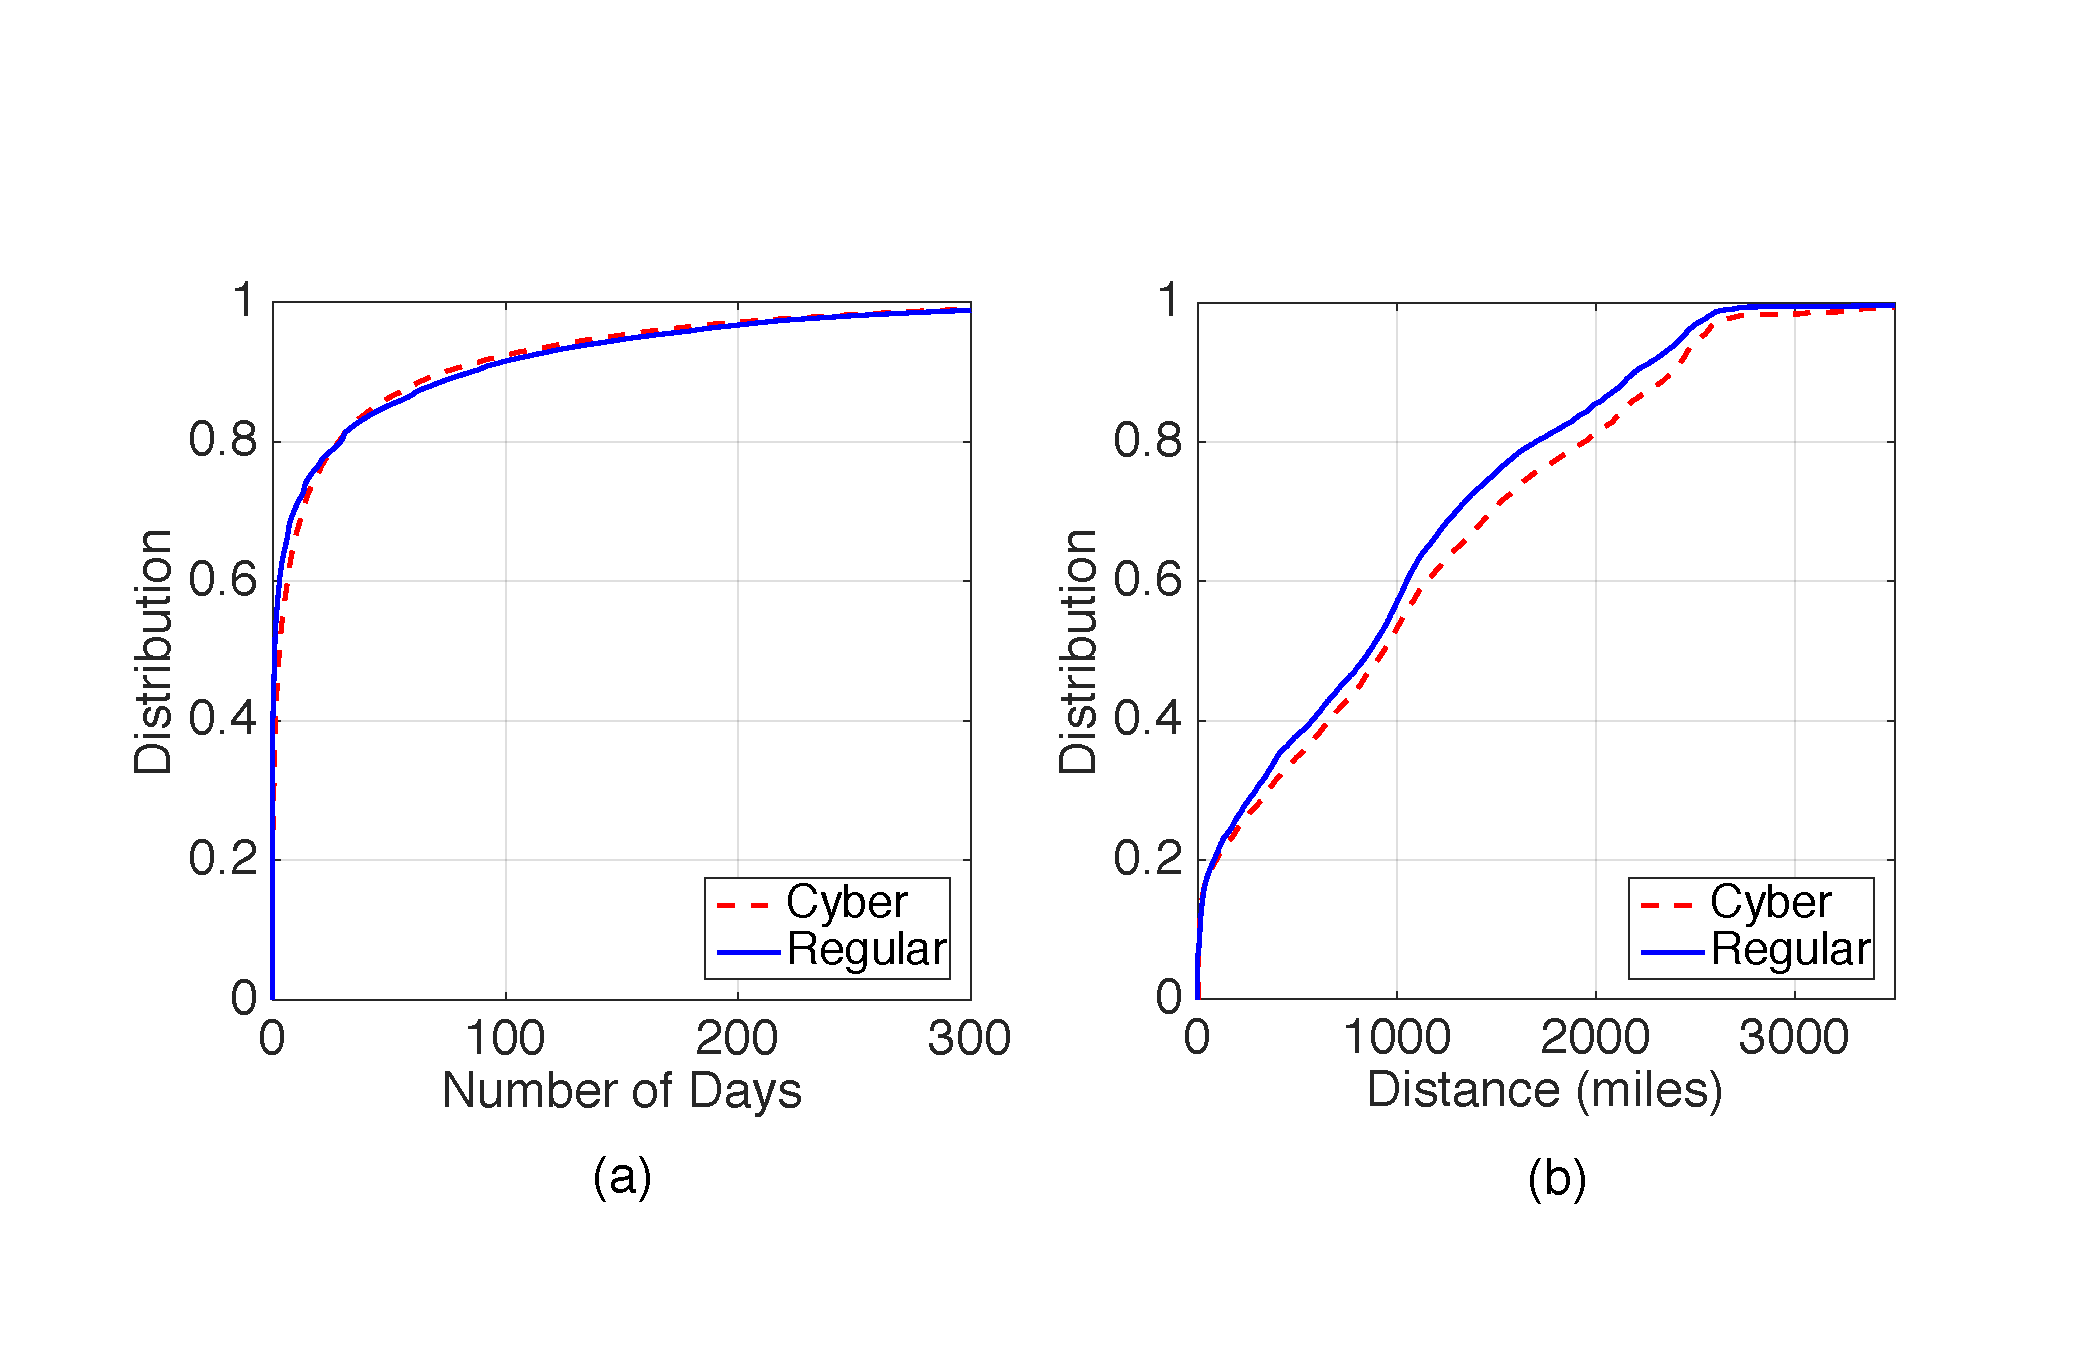
\includegraphics[scale=0.28]{graphics/dist_days.pdf}
  \caption{The cumulative distribution for (a) The difference between fraud and reporting dates. (b) The distance between consumers and fraudsters.}
  \label{cdffig}
\end{figure}


\subsection{Most Common Frauds}\label{fraudsters}

By using the fraud description fields we summarize the the top frauds in table 

\ref{topfrauds} provides a summary of the top frauds in each category.



We see a significant cyber presence of impostor scams and sweepstakes. While these frauds have long existed in the regular domain, this provides us anecdotal evidence that fraudsters are adopting new technology to execute the same types of scams online, which were previously perpetrated offline. We incorporate this specific insight in our discussion. Our results greatly align with the top sources of frauds stated in an FTC news release in 2016 \cite{ftcpress2016}. 


\subsection{Fraudster Coverage}\label{fraudstercoverage}

In order to understand the operational regions of fraudulent entities, we calculate the distances between consumer and fraudster zip codes. Figure \ref{cdffig} (b) provides a cumulative distribution of the operational radii for cyber and regular fraudsters.  This analysis provides insight on whether cyber fraudsters leverage the Internet for more visibility and access to target more distant individuals. With a median distance of 993 and 861 for cyber and regular frauds, we believe that both types of fraudsters follow similar trends. This indicates that Internet-based communication does not provide cyber fraudsters with a significant advantage over regular ones, as they are able to achieve similar operational spans by using phone and mail based communication methods.



\begin{table}[h]
\centering
\begin{tabular}{c|c|c}
\hline
\bfseries Metropolitan Area (MSA) & \bfseries \% Cyber & \bfseries \% Regular\\
\hline
\hline
New York, New Jersey, Long Island & 8.41 & 7.67 \\
\hline
Los Angeles, Long Beach, Santa Ana & 6.50 & 7.09 \\
\hline
Washington, Arlington, Alexandria & 4.10 & 5.78 \\
\hline
Miami-Fort Lauderdale, Pompano Beach & 4.16 & 5.40 \\
\hline
Dallas, Fort Worth, Arlington & 2.89 & 3.36\\
\hline
Chicago, Naperville Joliet & 3.17 & 3.27 \\
\hline
\end{tabular}
\vspace{8pt}
\caption{Top Fraudsters Locations}\label{topareas}
\vspace{-15pt}
\end{table}


\subsection{Top Fraudster Locations}\label{fraudser_locations}
Next, we identify the primary locations of the fraudsters within the United States and present our findings in \ref{topareas}. While fraudulent entities are spread throughout, most of the heavy hitters belong to the metropolitan areas. We believe this provides an efficient disguise to the fraudulent entities. We also observe certain areas that having a high cyber to regular fraud ratio and vice versa. The San Franciso, Oakland and San Jose, Santa Clara MSAs have a cyber to regular fraud ratio of 2.21 and 5.13. The popular fraud types in these regions are Internet services, unsolicited email, and online shopping. These areas serve as a good medium for cyber fraudsters as it allows them to gel into the surrounding cyber industry. Meanwhile, The Buffalo, Niagara Falls MSA has a regular to cyber fraud ratio of 8.76 with debt collection being the significant outlier. Further investigation reveals that Buffalo has a network of debt collectors which have been responsible for multi-million frauds \cite{buffalodebt1, buffalodebt2}.



\subsection{Demographic Analysis}\label{demographic_analysis}


By normalizing over cyber and regular frauds in each zip code, we evaluate how they vary with certain demographic features, which are obtained from the complementary datasets that we discuss in section \ref{data-cal}. 

To realize the effect of these features, we perform a logistic regression and summarize our coefficients and their significances in table \ref{regressions}. Among different ethnicities, only Hispanic communities show statistically significant change for cyber and regular fraud per capita. While the regression coefficients suggest that frauds decrease for heavier concentrations of  Hispanics, a survey study \cite{anderson2013consumer} showed that Hispanics and Black communities are more likely to be victims of crimes. The decreasing trend is likely a result of fraud under-reporting due to cultural reasons, distrust in institutions, and lack of awareness or education \cite{consumerlessons}.


Other socio-economic variables that we take into account are age, income, education, and unemployment rate. In addition to the regression analysis, we investigate their variation by observing complaint rates across their distributions in figure \ref{demographics}.

\textbf{Age:} While the differences in cyber and regular complaints remain fairly consistent, from figure \ref{demographics} (a) we observe that individuals greater that 50 years complain significantly more than other age groups. Our significant regression values also corroborate to this trend. 


\textbf{Education:} Both cyber and regular complaints increase along with an increase in percentage education. We associate this trend with greater increased educational awareness among individuals \cite{consumerlessons}. Another subtle trend, in the increase in cyber to regular complaint ratio from 0.82 to 1.23. We associate this diverging trend to more educated individuals being active on the Internet, and hence being more prone to online fraud~\cite{pewcollege}.

We do not include income and unemployment in our analysis due to their insignificant correlation values in table \ref{regressions}.

\begin{figure}[t]
\centering
  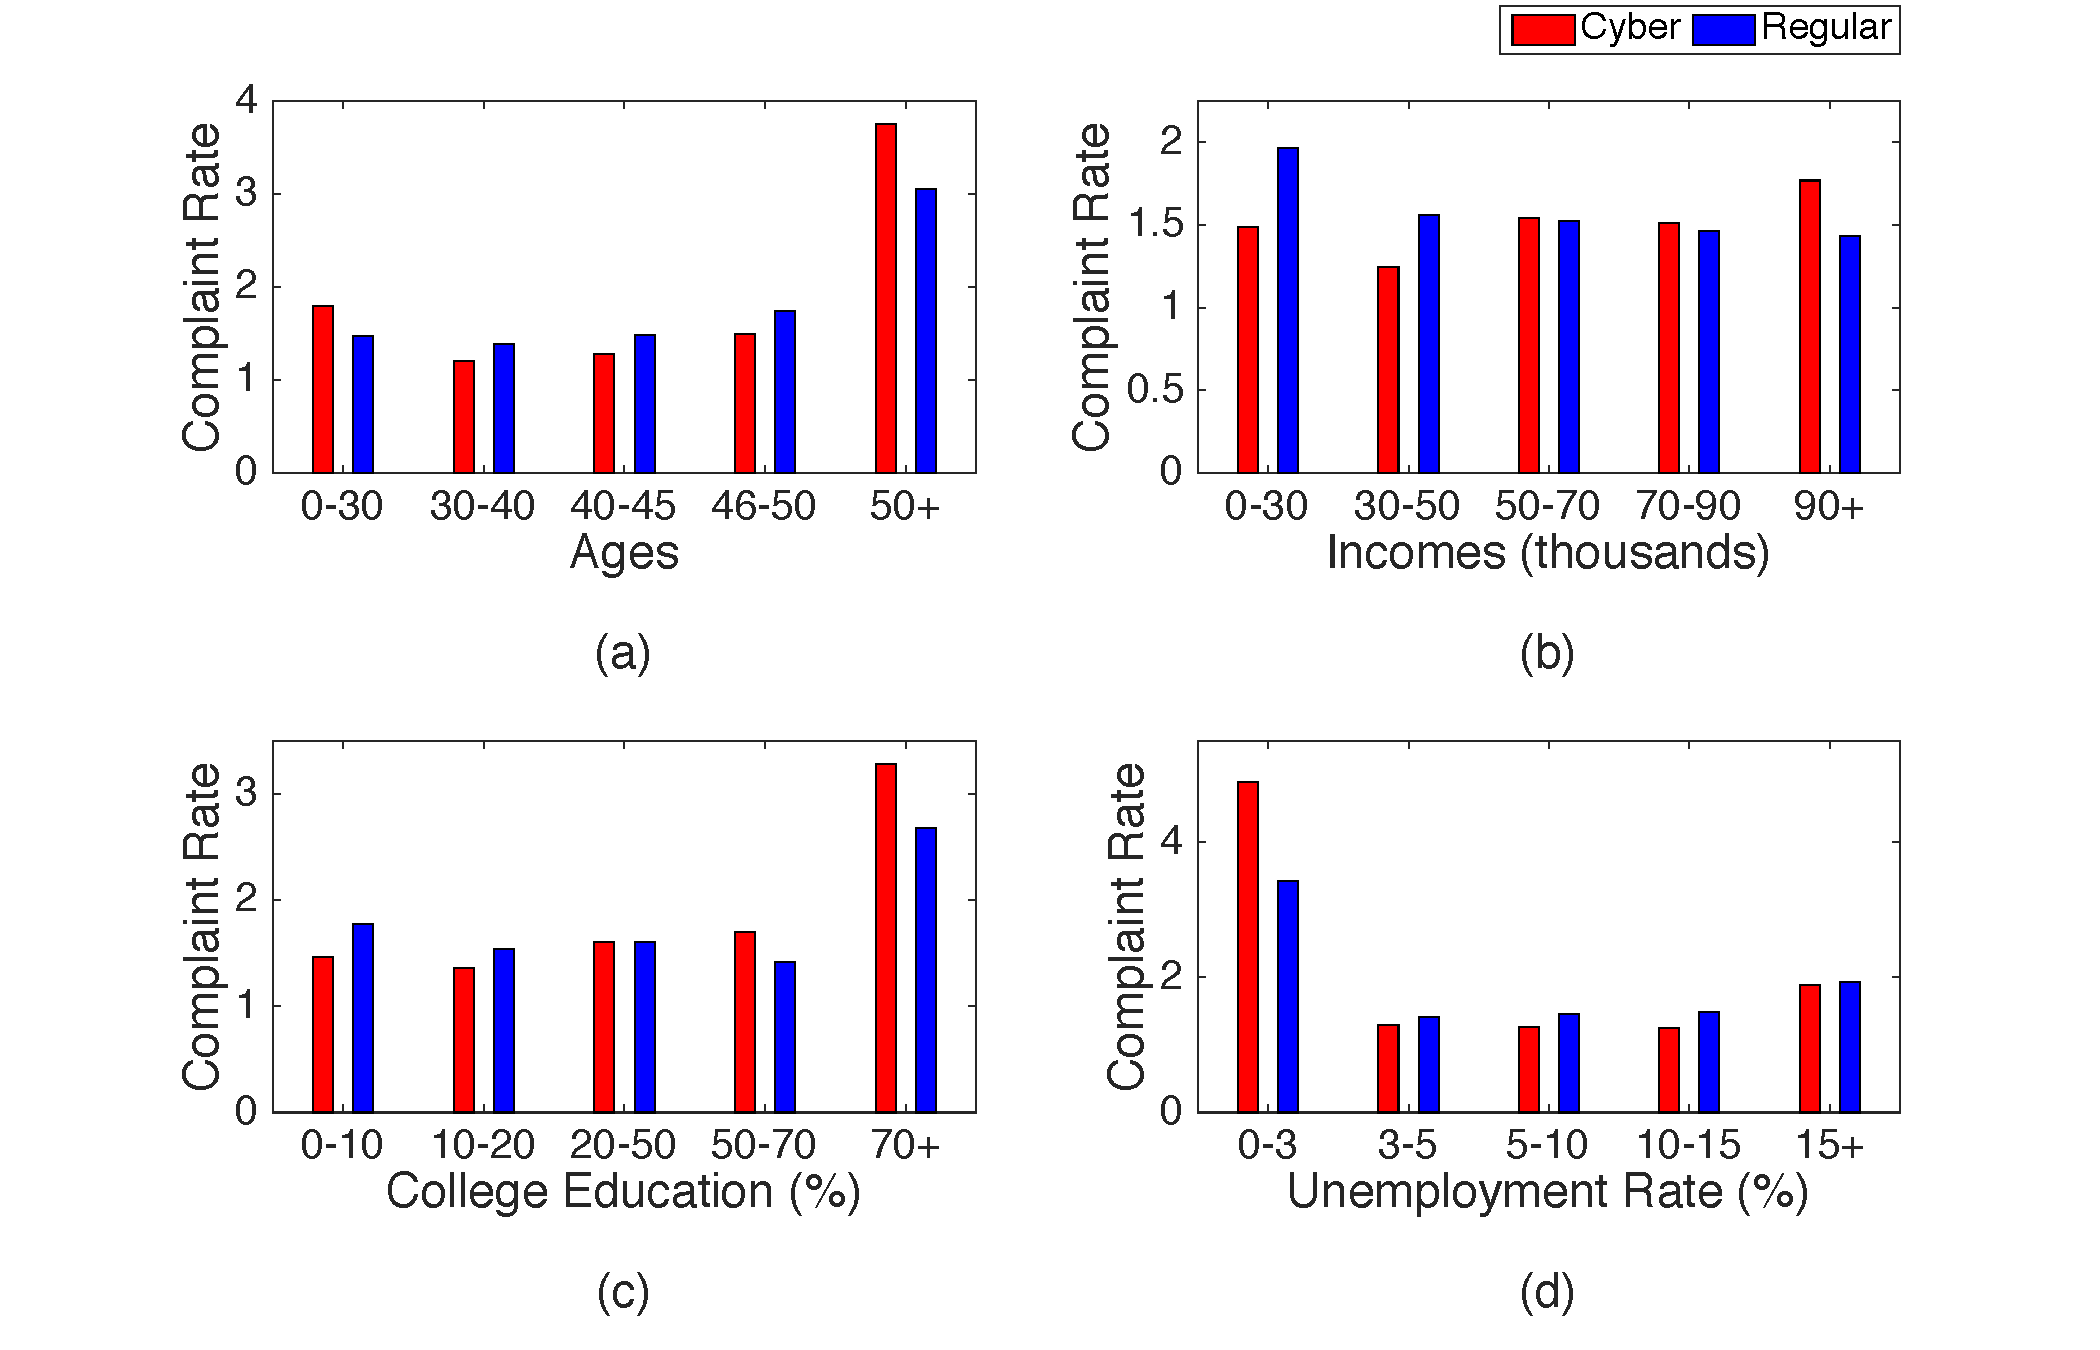
\includegraphics[scale=0.29]{graphics/demographics.pdf}
  \caption{Cyber and regular fraud trends over age, income, education and unemployment.}
  \label{demographics}
\end{figure}



\begin{table*}[h]
\noindent
\centering
\begin{tabular}{c||c|c|c||c|c|c}
\hline
\multicolumn{1}{c||}{\bfseries } & \multicolumn{3}{c||}{\bfseries Cyber Complaints Per Capita} & \multicolumn{3}{c}{\bfseries Regular Complaints Per Capita}\\
\hline
\bfseries Observed Variable & \bfseries Coefficient & \bfseries \emph{p-value} & \bfseries 95\% Confidence Interval & \bfseries Coefficient & \bfseries \emph{p-value} & \bfseries 95\% Confidence Interval \\
\hline
\% White (Non-Hispanic) & -0.0042 & 0.074 & [-0.009, 0] & -0.0013 &  0.128 & [0.003,  0]\\
\hline
\% Black & -0.0058 & 0.017 & [-0.011, -0.001] & 0.0017 & 0.054 & [-2.77$^{-5}$, -0.003]\\
\hline
\% Asian & -0.0025 & 0.468 & [-0.009, 0.004] & -0.0051 & 0.00 & [-0.008, -0.003]\\
\hline
\% Hispanic & -0.0026 & 0.014 & [-0.05, -0.001] & -0.0054 & 0.00 & [-0.006, -0.005]\\
\hline
Age & 0.0064 & 0.023 & [ 0.001, 0.012] & 0.0281 & 0.00 & [0.026, 0.030]\\
\hline
Income & -2.226$^{-6}$ & 8.85$^{-7}$ & [-3.96$^{-6}$ , -4.92$^{-7}$] & -3.695$^{-6}$ & 0.000  & [-4.31$^{-6}$, -3.08$^{-6}$]\\
\hline
Education & 0.0155 & 0.000 & [0.013, 0.018] & 0.0044 & 0.00 & [0.003, -0.005]\\
\hline
Unemployment & 0.0084 & 0.111 & [-0.002, 0.019] & -0.0028 & 0.138 & [-0.006, 0.001]\\
\hline
\end{tabular}
\vspace{8pt}
\caption{Regression Results for Per capita frauds evaluated for Ethnic and Socio-Economic factors}\label{regressions}
\vspace{-20pt}
\end{table*}

\section{Discussion}\label{discussion}
Based on our findings from section \ref{eval}, we elaborate some discussion points to provide context for this analysis in hopes that it will assist in the development of better policies and help reduce consumer fraud in the U.S. 

Our results indicate that while cyber frauds are on the rise, regular fraud methods still hold an equally significant share in the economy, and while policy developments are trending towards mitigating online fraud, there should be continuous awareness campaigns for phone, mail and other regular fraud types. As a result of reduced operational hours in the winter holidays, offline collection agencies experience an uneven decrease followed by a great influx of reports on resuming operation. To streamline the process, online reporting methods should be promoted.

We also learn that fraudulent entities tend to work in groups and establish networks \cite{buffalodebt2}. The fraudulent cyber establishments of San Jose and San Francisco discussed in Section \ref{fraudsters}, help us understand that fraudulent entities likely reflect the makeup of nearby legitimate industries.  

By observing the overlap between top cyber and regular frauds (Table \ref{topfrauds}) we realize that with the rise of Internet, fraudsters have their choice of vectors to execute scams that were traditionally only perpetrated through traditional means. Better understanding these advanced communication modalities requires a technologists' touch;  policy makers should consider working closely with technologists to devise detection mechanisms similar to \cite{brause1999neural, moreau1997detection} which enable better filtering and control of the fraudulent activity.

\section{Conclusion \& Future Work}\label{conclusion}

The goal of this paper is to investigate the dynamics of cyber and traditional methods for committing fraud in the United States. By partitioning the FTC Consumer Sentinel complaint dataset, we are able to explore trends among cyber and regular fraud, and analyze trends along time, distance and location metrics as well as their variation across consumer demographics. While the Internet has greatly expanded the potential reach and scale of fraudsters: where once they could only use mail or telephones for various frauds, the Internet enables one to contact millions of users very quickly, whether through fraudulent websites, Craigslist posts, or spam emails. Even so, the difference between the cyber and non-cyber methodologies is not overwhelming: this effect suggests that non-cyber activities, like purchasing goods or posting money orders, may still serve as a limiting factor on the extent or targeting of these fraudulent activities. 

Fraud analysis is an impactful topic that has been understudied in academia. While our current work has its limitations, we plan to extend our analysis over multiple years by establishing a collaboration with the FTC and obtaining high fidelity datasets that span a longer duration. We also look forward to evaluating our current findings with data collected by other regulatory agencies such as the FBI. This will eventually also allow us to overcome certain nuances and limitations of the current evaluation and help us develop stronger insights. Another interesting future direction is to evaluate how international fraud compares to fraud within the US, and identify any prominent international fraudsters who target US victims. This can possibly be achieved by using data from the European Commission and the eCrime project.


\section{Acknowledgments}\label{Acknowledgments}

We would like to thank the reviewers of the workshop for
reviewing our work and providing helpful feedback.


\bibliographystyle{IEEEtran}

\bibliography{references} 


% that's all folks
\end{document}


